% ============================================================
% 1D
% ============================================================

\section{Task 1D: Combined Optimization}

\subsection{Combined Optimization}
For our final optimized implementation, we combined five techniques:
\begin{enumerate}
    \item \textbf{Cache Tiling:} We blocked the output matrix into $32 \times 32$ spatial tiles (\texttt{oyT}, \texttt{oxT}) to restrict the active memory working set .
    \item \textbf{Loop Reordering:} Within each tile, we inverted the naive loop order to \texttt{ky} $\rightarrow$ \texttt{kx} $\rightarrow$ \texttt{oy} $\rightarrow$ \texttt{ox}, ensuring that the innermost memory accesses across the \texttt{ox} dimension are perfectly sequential .
    \item \textbf{SIMD Vectorization (AVX2):} We parallelized the innermost \texttt{ox} loop using 256-bit AVX2 vectors (\texttt{\_mm256\_loadu\_ps} and \texttt{\_mm256\_fmadd\_ps}), processing 8 pixels simultaneously .
    \item \textbf{Loop Unrolling (\texttt{kx}):} We unrolled the inner \texttt{kx} loop by a factor of 2, handling two adjacent kernel columns per iteration to further reduce branch overhead .
    \item \textbf{Multiple Independent Accumulators:} Inside the vector loop, we unrolled the \texttt{oy} dimension by 4, utilizing 4 independent AVX2 accumulators (\texttt{acc0} to \texttt{acc3}) to process a $4 \times 8$ block of output pixels simultaneously, maximizing instruction-level parallelism .
\end{enumerate}

\subsection{Why Combine These Techniques?}
The techniques address different parts of the execution. Tiling improves temporal locality and increases the chance that reused data are served from the cache hierarchy. Reordering makes the innermost \texttt{ox} accesses unit-stride, while SIMD increases the amount of arithmetic performed per vector instruction. Loop unrolling and multiple accumulators reduce loop-control work and expose independent operations. The measured combined speedup reflects their joint effect; it does not isolate a single bottleneck.

\subsection{Final Performance Comparison}

\begin{figure}[H]
    \centering
    \begin{subfigure}{0.85\textwidth}
        \centering
        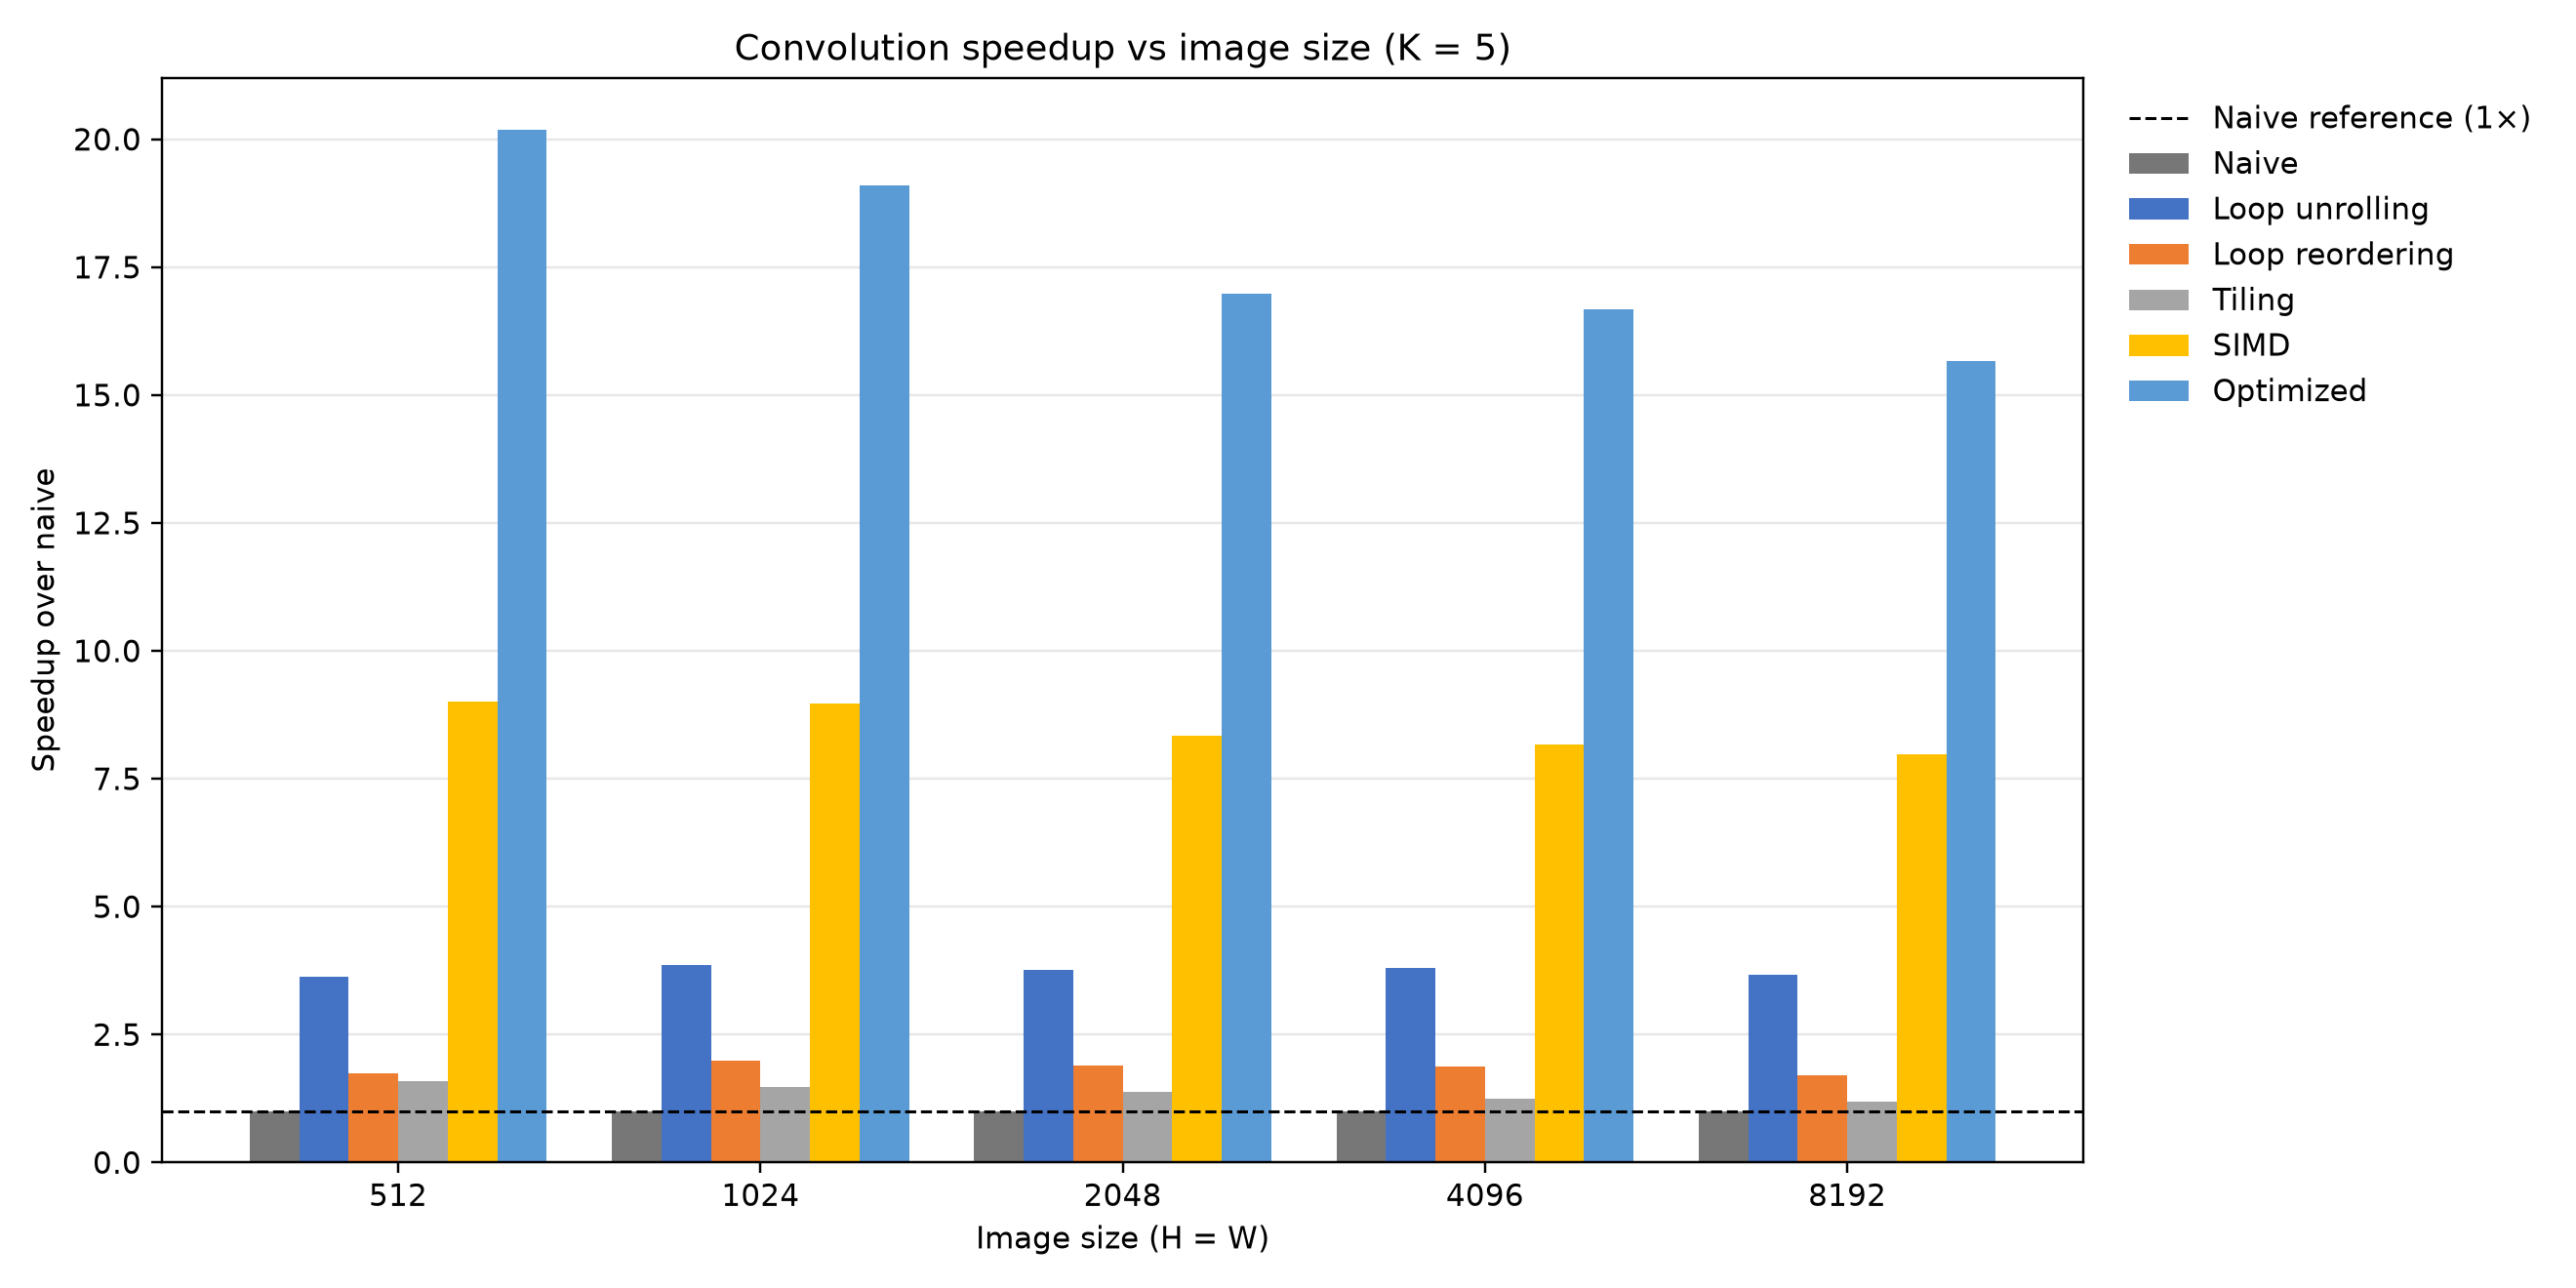
\includegraphics[width=\linewidth]{plots/task1d/speedup_vs_image_size.png}
        \caption{Speedup vs. Image Size ($K=5$)}
        \label{fig:task1d_image_size}
    \end{subfigure}
    
    \begin{subfigure}{0.85\textwidth}
        \centering
        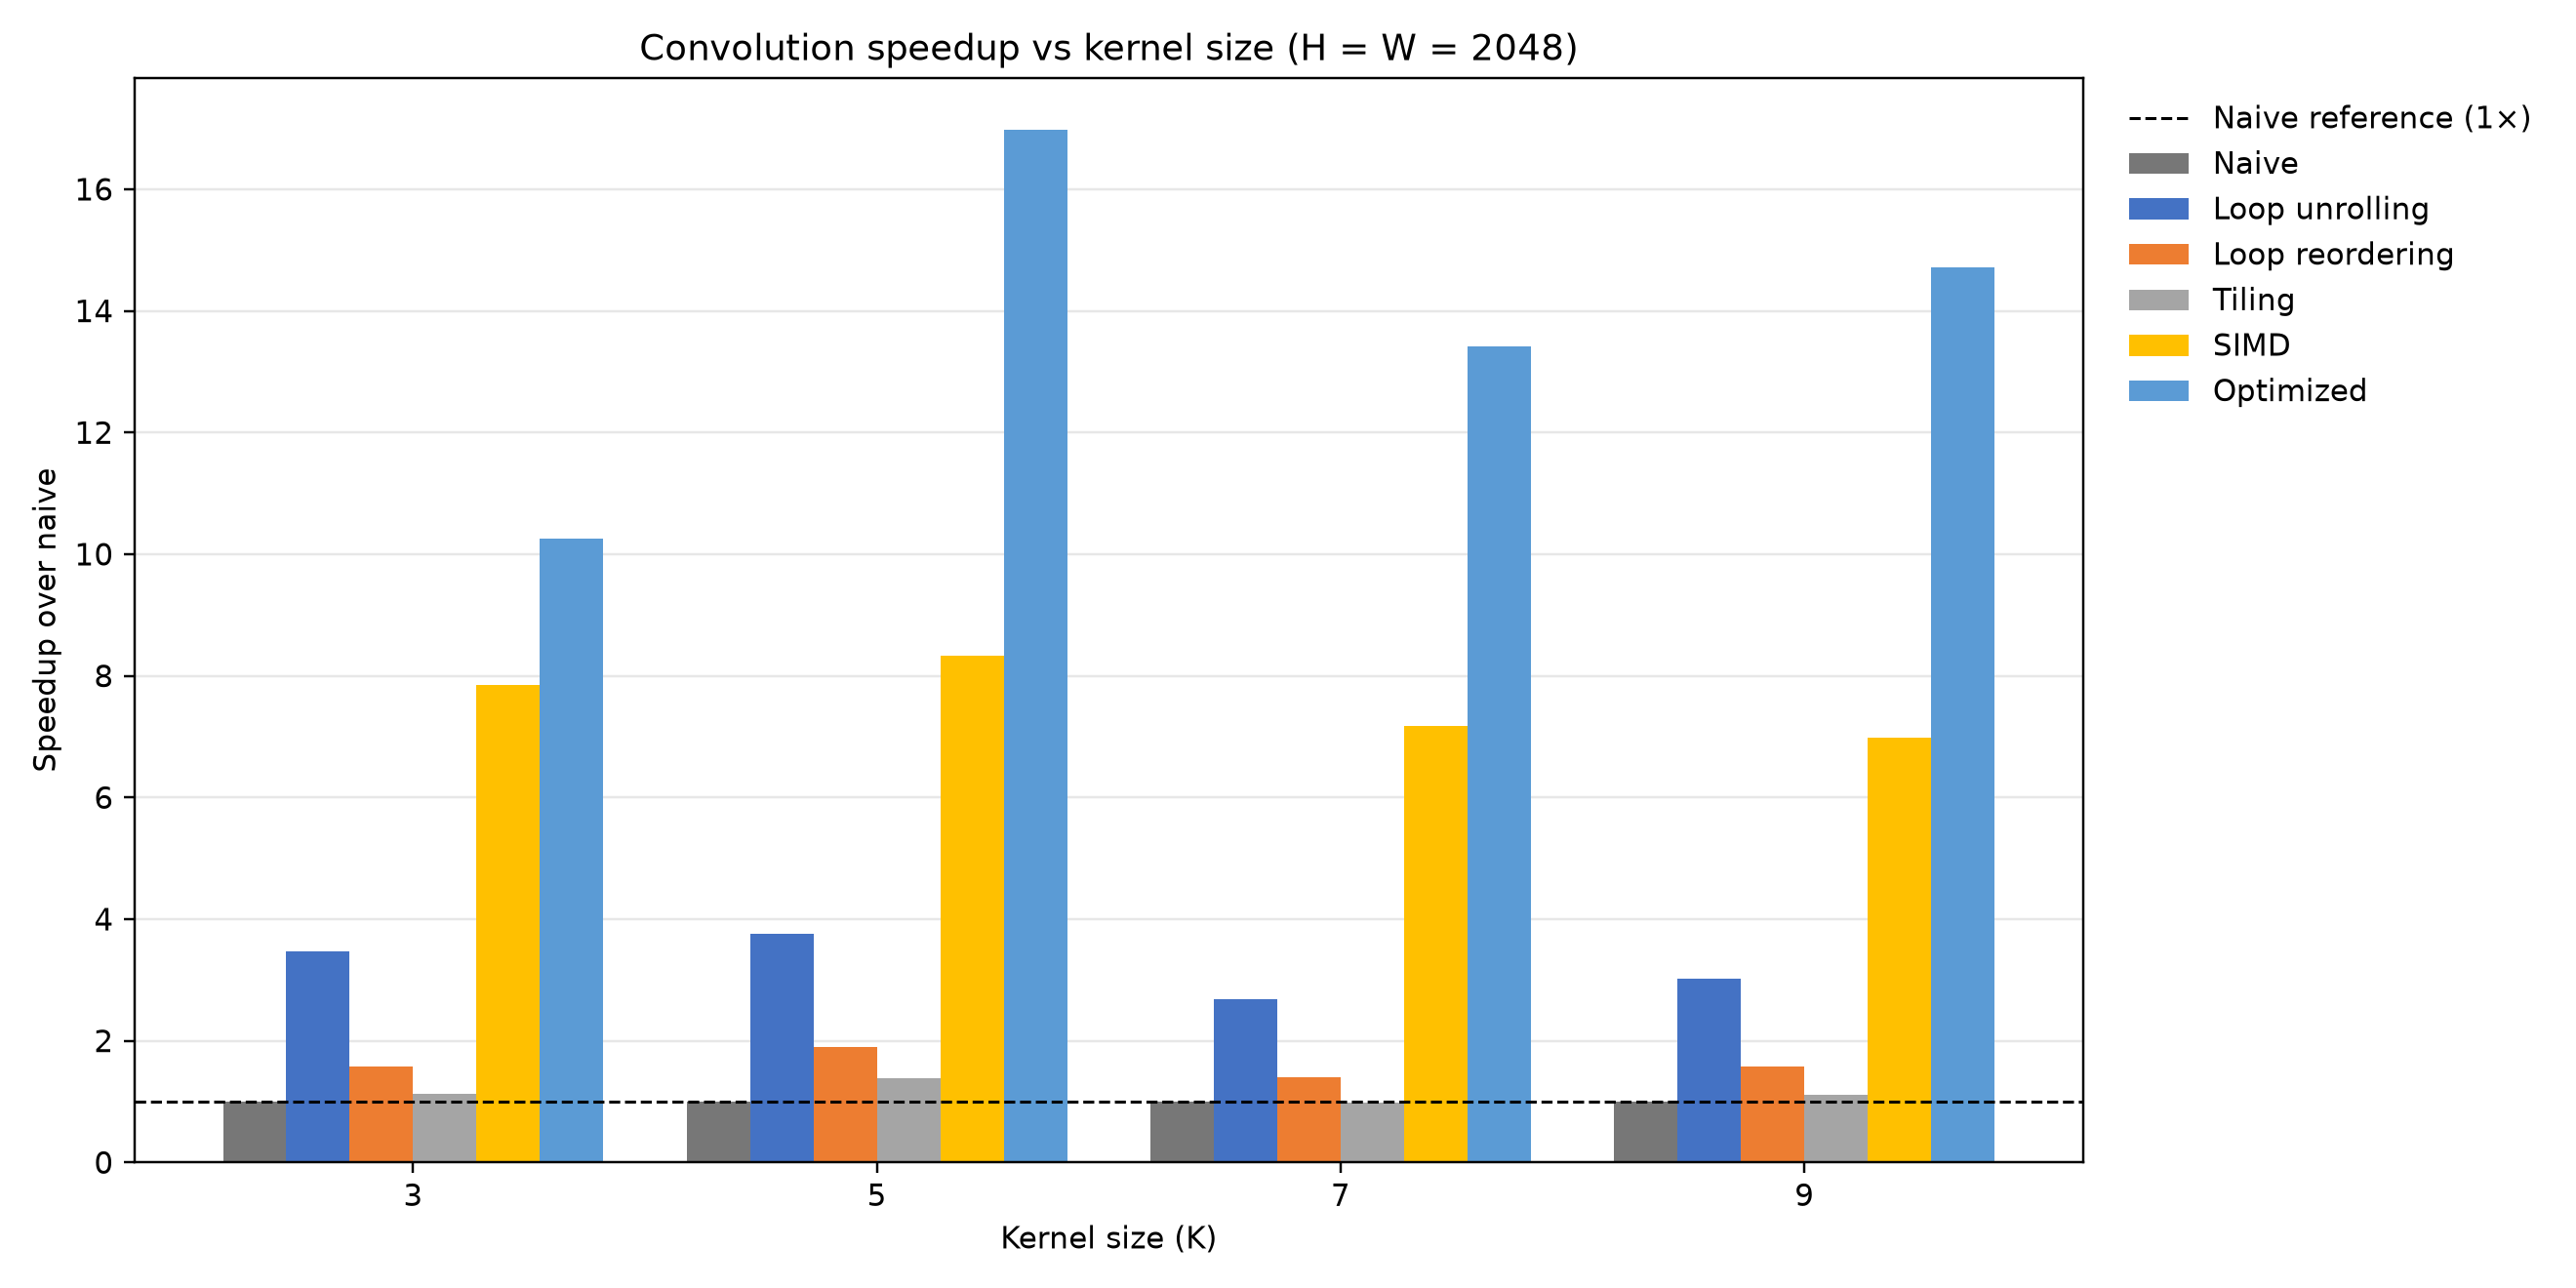
\includegraphics[width=\linewidth]{plots/task1d/speedup_vs_kernel_size.png}
        \caption{Speedup vs. Kernel Size ($2048 \times 2048$)}
        \label{fig:task1d_kernel_size}
    \end{subfigure}
    \caption{Best performance of the Task 1 optimization techniques.}
    \label{fig:task1_final_comparison}
\end{figure}

\begin{table}[H]
\centering
\caption{Task 1 final performance summary}
\begin{tabular}{lccl}
\toprule
Technique & Best Speedup & Workload & Primary Hardware Target \\
\midrule
Tiling & 1.60$\times$ & $512 \times 512, K=5$ & Cache capacity / L2+LLC hit rate \\
Loop reordering & 1.99$\times$ & $1024 \times 1024, K=5$ & Spatial locality / Hardware prefetching \\
Loop unrolling & 3.85$\times$ & $1024 \times 1024, K=5$ & Branch prediction / Loop overhead \\
SIMD (AVX2) & 9.01$\times$ & $512 \times 512, K=5$ & ALU saturation / Data parallelism \\
\textbf{Optimized (All Combined)} & \textbf{20.19$\times$} & $512 \times 512, K=5$ & \textbf{Cache locality / SIMD} \\
\bottomrule
\end{tabular}
\end{table}

\subsection{Discussion}
The combined implementation reaches a peak speedup of $20.19\times$, compared with the best isolated SIMD result of $9.01\times$. This improvement is consistent with combining vector arithmetic with improved locality and reduced loop overhead. The measurements show the combined effect, but do not by themselves prove that one specific memory bottleneck was eliminated or that the vector units reached a theoretical limit.

\subsection{Task 1 Conclusion}
Task 1 shows that loop structure and data layout matter alongside arithmetic complexity. Reordering improves unit-stride access, tiling improves reuse over a limited working set, unrolling reduces loop-control work and exposes independent operations, and SIMD raises the amount of work per vector instruction. Their combination produced the best result on the measured workloads.
